\documentclass[11pt,a4paper]{article}
\usepackage[margin=1in]{geometry}
\usepackage{booktabs,graphicx,float,hyperref,xcolor,amsmath}
\usepackage[default]{sourcesanspro}
\hypersetup{colorlinks=true,linkcolor=blue,urlcolor=blue}
\title{ECG5000 Anomaly Detection\\\large A Normal-Only Conv1D and LSTM Autoencoder Comparison}
\author{Mohammad Torabi \\ 404422041}
\date{Course: Data Mining \\ Instructor: Dr. Hadi Farahani \\ August 2026}
\begin{document}
\maketitle
\begin{abstract}
This project detects anomalous heartbeats with autoencoders trained only on normal ECG signals. My contribution is a controlled comparison between a Conv1D autoencoder and an LSTM autoencoder, using the same normal-only split and the same robust threshold rule. On the held-out test set, Conv1D-AE gives the best F1 score (0.912), while LSTM-AE gives slightly higher recall (0.997). The results show a clear precision--recall trade-off.
\end{abstract}

\section{Problem and Data}
ECG5000 has 5,000 univariate heartbeat sequences, each with 140 time steps and one of five original labels. I treat label 1 as normal and labels 2--5 as anomalous. The given split has 500 training examples and 4,500 test examples. Only normal examples from the training part are used to fit the models. I reserve 20\% of these normal training beats for validation with seed 42, and I keep the full original test split for final evaluation.

\begin{figure}[H]\centering

\includegraphics[width=.72\linewidth]{figures/class_balance.png}
\caption{Normal and anomalous beats are imbalanced, so accuracy alone would be misleading.}\label{fig:balance}
\end{figure}
\begin{figure}[H]\centering
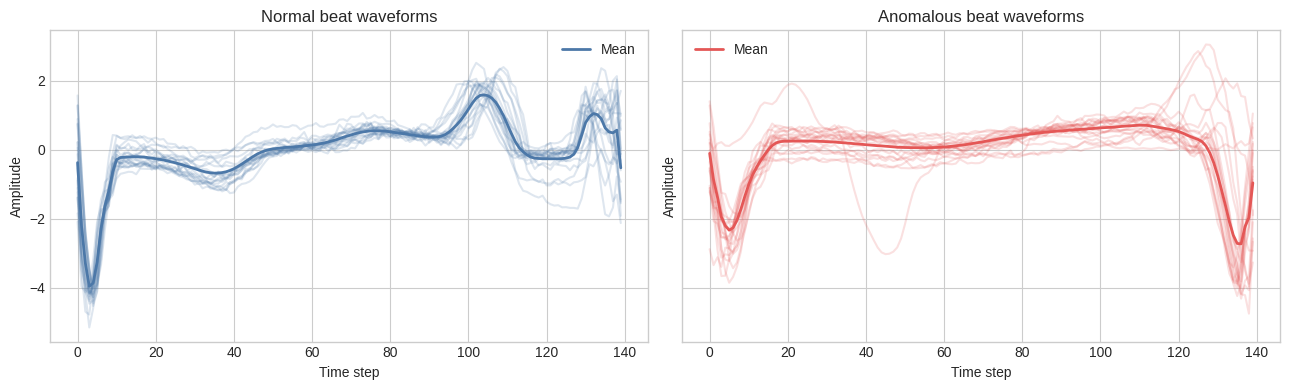
\includegraphics[width=\linewidth]{figures/waveforms.png}
\caption{Examples of normal and anomalous waveform distributions.}\label{fig:waveforms}
\end{figure}

\section{Method and Original Contribution}
Both models minimize mean squared reconstruction error on normal beats only. Conv1D-AE uses two strided convolutional encoder stages with transpose-convolution decoding. LSTM-AE uses encoder and decoder LSTMs. Both have a 16-dimensional bottleneck, AdamW, the same batch size, validation split, and seed.

Instead of selecting a fixed percentile, I set each anomaly threshold from the held-out normal validation errors:
\[
\tau=\operatorname{median}(e_{val})+3\times1.4826\times\operatorname{MAD}(e_{val}).
\]
This median absolute deviation (MAD) rule is robust to unusually difficult normal beats. A test beat is anomalous when its reconstruction MSE is above $\tau$. The true anomaly labels are not used for threshold selection.

\section{Real Results and Analysis}
Table~\ref{tab:results} uses the saved output in \path{outputs/results.csv}. Conv1D-AE has F1 of 0.912, precision of 0.842, and recall of 0.995. LSTM-AE has lower F1 (0.891) and precision (0.805), but it misses only 5 anomalies instead of 10. In contrast, LSTM-AE produces 452 false positives while Conv1D-AE produces 349. For this experiment, Conv1D-AE is the more balanced detector, while LSTM-AE is preferable only if missing an anomaly is more costly than additional alarms.

\begin{table}[H]\centering
\caption{Held-out test results and thresholds from the saved experiment.}\label{tab:results}
\begin{tabular}{lrrrrrr}
\toprule
Model & Threshold & Precision & Recall & F1 & AP & ROC-AUC \\
\midrule
Conv1D-AE & 1.3548 & \textbf{0.842} & 0.995 & \textbf{0.912} & \textbf{0.851} & 0.950 \\
LSTM-AE & 1.0754 & 0.805 & \textbf{0.997} & 0.891 & 0.851 & \textbf{0.950} \\
\bottomrule
\end{tabular}
\end{table}
\begin{figure}[H]\centering
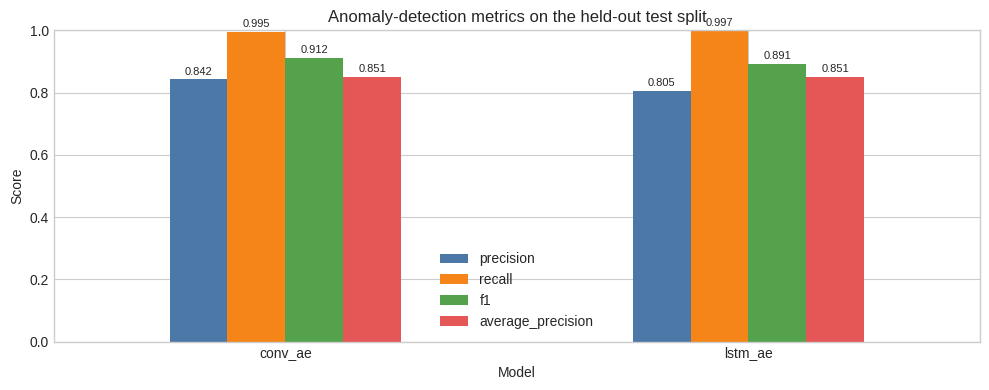
\includegraphics[width=\linewidth]{figures/metrics.png}
\caption{Precision, recall, F1, and average precision for both models.}\label{fig:metrics}
\end{figure}
\begin{figure}[H]\centering
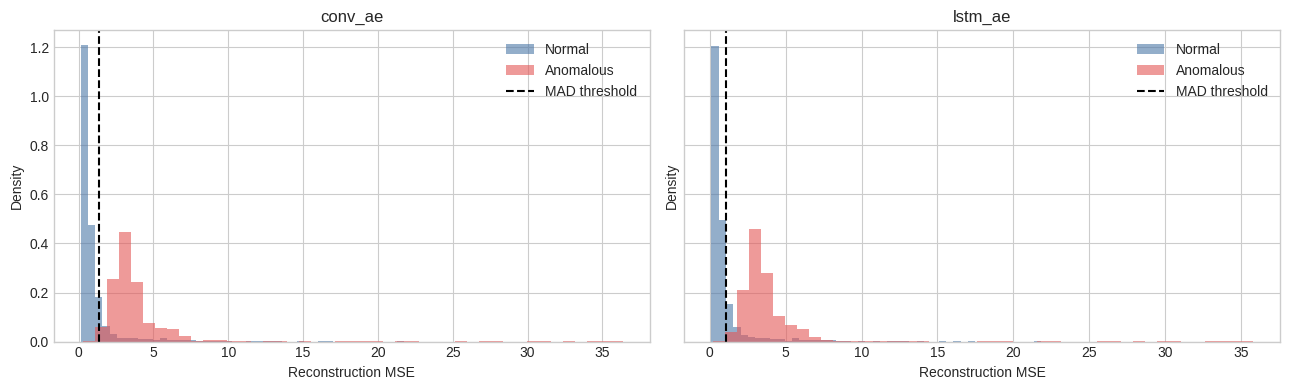
\includegraphics[width=\linewidth]{figures/error_distributions.png}
\caption{Reconstruction-error distributions and the MAD thresholds.}\label{fig:errors}
\end{figure}

\section{Failure Analysis and Limitations}
A normal beat can be falsely flagged when its amplitude or timing pattern is uncommon in the normal-only training subset. A false negative can happen when an anomalous morphology is reconstructed too well. Figure~\ref{fig:demo} shows saved original/reconstructed examples, which helps to inspect this behavior.
\begin{figure}[H]\centering
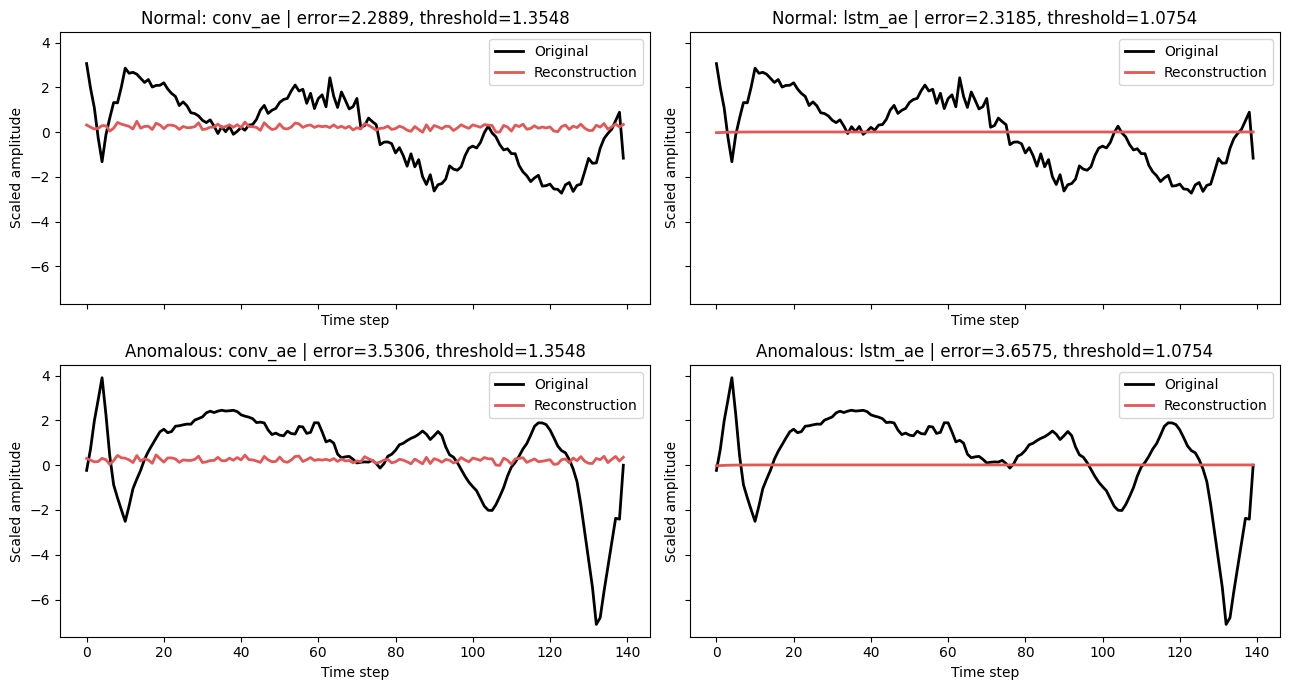
\includegraphics[width=\linewidth]{figures/reconstructions.png}
\caption{Saved reconstructions for normal and anomalous test beats.}\label{fig:demo}
\end{figure}

These are one-epoch CPU verification results, so I should not claim that one architecture always wins. Future work should repeat several seeds, report results for each raw anomaly label, and compare with a one-class classical baseline. This would show whether the difference is stable and which morphology types are difficult.

\section{Discussion and Observation}
\subsection*{The over-capable autoencoder paradox}
If an autoencoder has too much capacity, it may learn to reconstruct anomalous beats almost as well as normal beats. Then the reconstruction errors overlap and anomaly detection becomes weak. I try to reduce this risk with a small 16-dimensional bottleneck, shallow models, early stopping, and normal-only training data. A larger model is not automatically better for this task.

\subsection*{Would self-attention help?}
Attention could show which time regions are used to form a normal heartbeat representation, for example a peak shape and the recovery region. However, there are only 140 time points and a small normal training set. For this reason, attention may only add parameters and overfit. I would add it only after testing whether the convolutional and LSTM models miss long-range waveform relations.

\section{Reproducibility}
Run \path{python scripts/train.py} from the project directory. It saves the metrics, error values, model weights, and demo arrays in \path{outputs/}. Then run the notebooks to recreate the report figures.
\end{document}
